\section*{Problem 2}
	\begin{proof}
		Just put $n = \frac{x}{\Delta x}, k = \frac{t}{\Delta t}$ into $p(n, k)$ and run brute-force calculation. Then we get the desired result:
		\begin{align*}
			p(n, k) = p(\frac{x}{\Delta x}, \frac{t}{\Delta t}) = 2\Delta x \cdot p(x, t)
		\end{align*}
		This model has only 2 choices: left and right. Let $m_i$ be a position at $i$th iteration. Let $N_l, N_r$ be a number of choices of left and right each. Then $m_i = m_0 - N_l + N_r = N_l + N_r$ and $N_l + N_r = i$, so
		\begin{align*}
			m_i + i &= 2N_r,\\
			i - m_i &= 2N_l
		\end{align*}
		This means if $i$ is even, then $m_i$ also even. So it is impossible to spread equally in odd places and even places, just one places have both. Therefore, the term $2\Delta x$ needs to explain this model well. To fix this, we need to add more variety to movement. We can use the 3-choice model instead of the 2-choice model.
		\begin{center}
			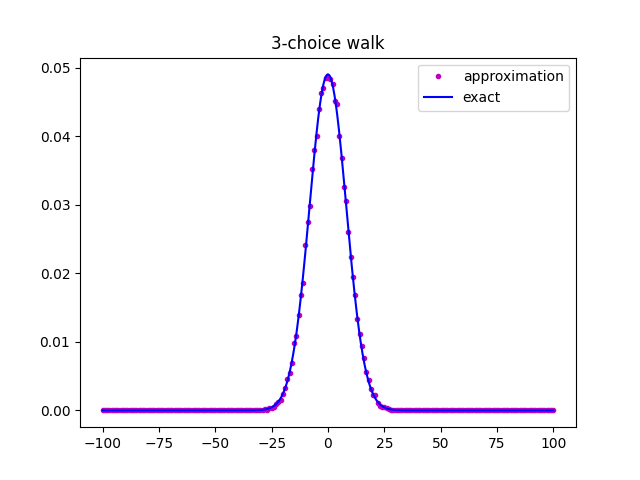
\includegraphics[width=0.7\textwidth]{3_and_var.png}
		\end{center}
	\end{proof}